\documentclass{standalone}
\usepackage{tikz}
\usetikzlibrary{patterns, positioning}


\begin{document}
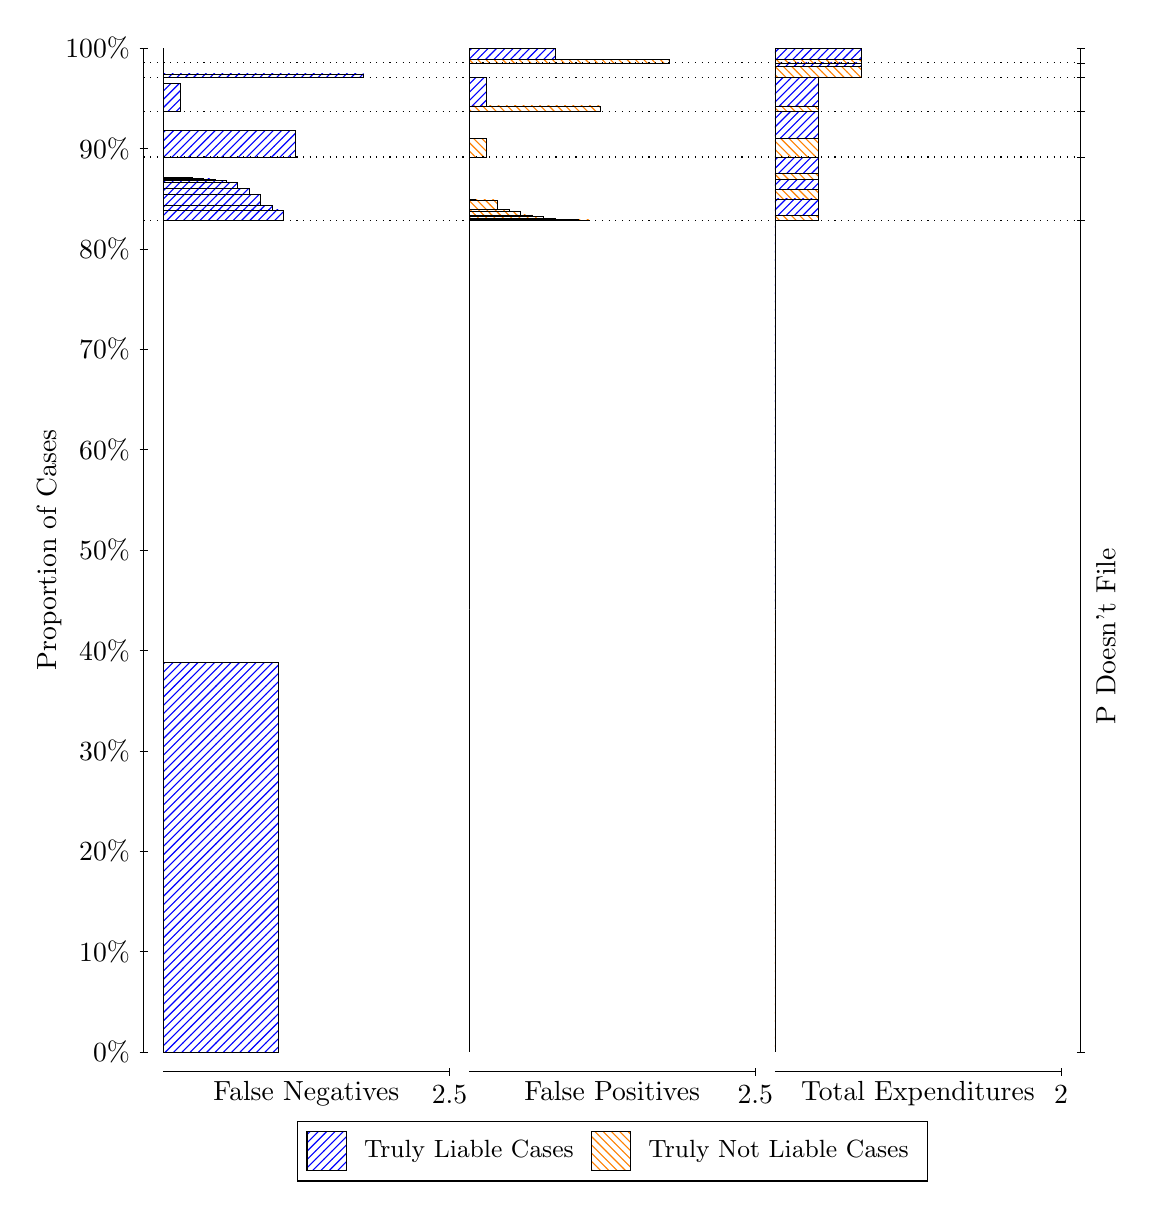
\begin{tikzpicture}
\draw[black, very thin] (1.5,1.75) -- (1.5,14.5);
\node[rotate=90, text=black, anchor=center] at (0.3, 8.125) {Proportion of Cases};
\draw[black, very thin] (1.45,1.75) -- (1.55,1.75);
\node[text=black, anchor=east] at (1.45, 1.75) {0\%};
\draw[black, very thin] (1.45,3.025) -- (1.55,3.025);
\node[text=black, anchor=east] at (1.45, 3.025) {10\%};
\draw[black, very thin] (1.45,4.3) -- (1.55,4.3);
\node[text=black, anchor=east] at (1.45, 4.3) {20\%};
\draw[black, very thin] (1.45,5.575) -- (1.55,5.575);
\node[text=black, anchor=east] at (1.45, 5.575) {30\%};
\draw[black, very thin] (1.45,6.85) -- (1.55,6.85);
\node[text=black, anchor=east] at (1.45, 6.85) {40\%};
\draw[black, very thin] (1.45,8.125) -- (1.55,8.125);
\node[text=black, anchor=east] at (1.45, 8.125) {50\%};
\draw[black, very thin] (1.45,9.4) -- (1.55,9.4);
\node[text=black, anchor=east] at (1.45, 9.4) {60\%};
\draw[black, very thin] (1.45,10.675) -- (1.55,10.675);
\node[text=black, anchor=east] at (1.45, 10.675) {70\%};
\draw[black, very thin] (1.45,11.95) -- (1.55,11.95);
\node[text=black, anchor=east] at (1.45, 11.95) {80\%};
\draw[black, very thin] (1.45,13.225) -- (1.55,13.225);
\node[text=black, anchor=east] at (1.45, 13.225) {90\%};
\draw[black, very thin] (1.45,14.5) -- (1.55,14.5);
\node[text=black, anchor=east] at (1.45, 14.5) {100\%};

\draw[black, very thin] (13.4,1.75) -- (13.4,14.5);
\draw[black, very thin] (13.35,1.75) -- (13.45,1.75);
\node[anchor=west] at (13.35, 1.75) {};
\draw[black, very thin] (13.35,12.313) -- (13.45,12.313);
\node[anchor=west] at (13.35, 12.313) {};
\draw[black, very thin] (13.35,13.116) -- (13.45,13.116);
\node[anchor=west] at (13.35, 13.116) {};
\draw[black, very thin] (13.35,13.692) -- (13.45,13.692);
\node[anchor=west] at (13.35, 13.692) {};
\draw[black, very thin] (13.35,14.123) -- (13.45,14.123);
\node[anchor=west] at (13.35, 14.123) {};
\draw[black, very thin] (13.35,14.311) -- (13.45,14.311);
\node[anchor=west] at (13.35, 14.311) {};
\draw[black, very thin] (13.35,14.5) -- (13.45,14.5);
\node[anchor=west] at (13.35, 14.5) {};

\draw[black, very thin, pattern color=blue, pattern=north east lines] (1.75,1.75) rectangle (3.2033,6.6952);
\draw[black, very thin, pattern color=orange, pattern=north west lines] (1.75,6.6952) rectangle (1.75,12.313);
\draw[black, very thin, pattern color=blue, pattern=north east lines] (1.75,12.313) rectangle (3.276,12.445);
\draw[black, very thin, pattern color=blue, pattern=north east lines] (1.75,12.445) rectangle (3.1307,12.505);
\draw[black, very thin, pattern color=blue, pattern=north east lines] (1.75,12.505) rectangle (2.9853,12.639);
\draw[black, very thin, pattern color=blue, pattern=north east lines] (1.75,12.639) rectangle (2.84,12.722);
\draw[black, very thin, pattern color=blue, pattern=north east lines] (1.75,12.722) rectangle (2.6947,12.796);
\draw[black, very thin, pattern color=blue, pattern=north east lines] (1.75,12.796) rectangle (2.5493,12.819);
\draw[black, very thin, pattern color=blue, pattern=north east lines] (1.75,12.819) rectangle (2.404,12.839);
\draw[black, very thin, pattern color=blue, pattern=north east lines] (1.75,12.839) rectangle (2.2587,12.849);
\draw[black, very thin, pattern color=blue, pattern=north east lines] (1.75,12.849) rectangle (2.1133,12.857);
\draw[black, very thin, pattern color=orange, pattern=north west lines] (1.75,12.857) rectangle (1.75,13.116);
\draw[black, very thin, pattern color=blue, pattern=north east lines] (1.75,13.116) rectangle (3.4213,13.453);
\draw[black, very thin, pattern color=orange, pattern=north west lines] (1.75,13.453) rectangle (1.75,13.692);
\draw[black, very thin, pattern color=blue, pattern=north east lines] (1.75,13.692) rectangle (1.968,14.05);
\draw[black, very thin, pattern color=orange, pattern=north west lines] (1.75,14.05) rectangle (1.75,14.123);
\draw[black, very thin, pattern color=blue, pattern=north east lines] (1.75,14.123) rectangle (4.2933,14.171);
\draw[black, very thin, pattern color=orange, pattern=north west lines] (1.75,14.171) rectangle (1.75,14.311);
\draw[black, very thin, pattern color=orange, pattern=north west lines] (1.75,14.311) rectangle (1.75,14.36);
\draw[black, very thin, pattern color=blue, pattern=north east lines] (1.75,14.36) rectangle (1.75,14.5);
\draw[black, very thin, pattern color=orange, pattern=north west lines] (5.6333,1.75) rectangle (5.6333,7.3673);
\draw[black, very thin, pattern color=blue, pattern=north east lines] (5.6333,7.3673) rectangle (5.6333,12.313);
\draw[black, very thin, pattern color=orange, pattern=north west lines] (5.6333,12.313) rectangle (7.1593,12.316);
\draw[black, very thin, pattern color=orange, pattern=north west lines] (5.6333,12.316) rectangle (7.014,12.319);
\draw[black, very thin, pattern color=orange, pattern=north west lines] (5.6333,12.319) rectangle (6.8687,12.326);
\draw[black, very thin, pattern color=orange, pattern=north west lines] (5.6333,12.326) rectangle (6.7233,12.335);
\draw[black, very thin, pattern color=orange, pattern=north west lines] (5.6333,12.335) rectangle (6.578,12.358);
\draw[black, very thin, pattern color=orange, pattern=north west lines] (5.6333,12.358) rectangle (6.4327,12.378);
\draw[black, very thin, pattern color=orange, pattern=north west lines] (5.6333,12.378) rectangle (6.4327,12.382);
\draw[black, very thin, pattern color=orange, pattern=north west lines] (5.6333,12.382) rectangle (6.2873,12.428);
\draw[black, very thin, pattern color=orange, pattern=north west lines] (5.6333,12.428) rectangle (6.142,12.454);
\draw[black, very thin, pattern color=orange, pattern=north west lines] (5.6333,12.454) rectangle (5.9967,12.571);
\draw[black, very thin, pattern color=blue, pattern=north east lines] (5.6333,12.571) rectangle (5.706,12.58);
\draw[black, very thin, pattern color=blue, pattern=north east lines] (5.6333,12.58) rectangle (5.6333,13.116);
\draw[black, very thin, pattern color=orange, pattern=north west lines] (5.6333,13.116) rectangle (5.8513,13.355);
\draw[black, very thin, pattern color=blue, pattern=north east lines] (5.6333,13.355) rectangle (5.6333,13.692);
\draw[black, very thin, pattern color=orange, pattern=north west lines] (5.6333,13.692) rectangle (7.3047,13.764);
\draw[black, very thin, pattern color=blue, pattern=north east lines] (5.6333,13.764) rectangle (5.8513,14.123);
\draw[black, very thin, pattern color=orange, pattern=north west lines] (5.6333,14.123) rectangle (5.6333,14.262);
\draw[black, very thin, pattern color=blue, pattern=north east lines] (5.6333,14.262) rectangle (5.6333,14.311);
\draw[black, very thin, pattern color=orange, pattern=north west lines] (5.6333,14.311) rectangle (8.1767,14.36);
\draw[black, very thin, pattern color=blue, pattern=north east lines] (5.6333,14.36) rectangle (6.7233,14.5);
\draw[black, very thin, pattern color=orange, pattern=north west lines] (9.5167,1.75) rectangle (9.5167,7.3673);
\draw[black, very thin, pattern color=blue, pattern=north east lines] (9.5167,7.3673) rectangle (9.5167,12.313);
\draw[black, very thin, pattern color=orange, pattern=north west lines] (9.5167,12.313) rectangle (10.062,12.378);
\draw[black, very thin, pattern color=blue, pattern=north east lines] (9.5167,12.378) rectangle (10.062,12.585);
\draw[black, very thin, pattern color=orange, pattern=north west lines] (9.5167,12.585) rectangle (10.062,12.702);
\draw[black, very thin, pattern color=blue, pattern=north east lines] (9.5167,12.702) rectangle (10.062,12.835);
\draw[black, very thin, pattern color=orange, pattern=north west lines] (9.5167,12.835) rectangle (10.062,12.911);
\draw[black, very thin, pattern color=blue, pattern=north east lines] (9.5167,12.911) rectangle (10.062,13.116);
\draw[black, very thin, pattern color=orange, pattern=north west lines] (9.5167,13.116) rectangle (10.062,13.355);
\draw[black, very thin, pattern color=blue, pattern=north east lines] (9.5167,13.355) rectangle (10.062,13.692);
\draw[black, very thin, pattern color=orange, pattern=north west lines] (9.5167,13.692) rectangle (10.062,13.764);
\draw[black, very thin, pattern color=blue, pattern=north east lines] (9.5167,13.764) rectangle (10.062,14.123);
\draw[black, very thin, pattern color=orange, pattern=north west lines] (9.5167,14.123) rectangle (10.607,14.262);
\draw[black, very thin, pattern color=blue, pattern=north east lines] (9.5167,14.262) rectangle (10.607,14.311);
\draw[black, very thin, pattern color=orange, pattern=north west lines] (9.5167,14.311) rectangle (10.607,14.36);
\draw[black, very thin, pattern color=blue, pattern=north east lines] (9.5167,14.36) rectangle (10.607,14.5);
\draw[black, dotted] (1.5,12.313) -- (13.4,12.313);
\draw[black, dotted] (1.5,13.116) -- (13.4,13.116);
\draw[black, dotted] (1.5,13.692) -- (13.4,13.692);
\draw[black, dotted] (1.5,14.123) -- (13.4,14.123);
\draw[black, dotted] (1.5,14.311) -- (13.4,14.311);
\draw[black, very thin] (1.75,1.5) -- (5.3833,1.5);
\node[text=black, anchor=north] at (3.5667, 1.5) {False Negatives};
\draw[black, very thin] (5.3833,1.45) -- (5.3833,1.55);
\node[text=black, anchor=north] at (5.3833, 1.45) {2.5};

\draw[black, very thin] (5.6333,1.5) -- (9.2667,1.5);
\node[text=black, anchor=north] at (7.45, 1.5) {False Positives};
\draw[black, very thin] (9.2667,1.45) -- (9.2667,1.55);
\node[text=black, anchor=north] at (9.2667, 1.45) {2.5};

\draw[black, very thin] (9.5167,1.5) -- (13.15,1.5);
\node[text=black, anchor=north] at (11.333, 1.5) {Total Expenditures};
\draw[black, very thin] (13.15,1.45) -- (13.15,1.55);
\node[text=black, anchor=north] at (13.15, 1.45) {2};

\node[text=black, centered, rotate=90] at (13.72, 7.0313) {P Doesn't File};






\draw (7.449999999999999,1.5) node[draw=none] (baseCoordinate) {};
\begin{scope}[align=center]
        \matrix[scale=0.5, draw=black, below=0.5cm of baseCoordinate, nodes={draw}, column sep=0.1cm]{
            \node[rectangle, draw, minimum width=0.5cm, minimum height=0.5cm, pattern color=blue, pattern=north east lines] {}; &
            \node[draw=none, font=\small, text=black] (B) {Truly Liable Cases}; &
            \node[rectangle, draw, minimum width=0.5cm, minimum height=0.5cm, pattern color=orange, pattern=north west lines] {}; &
            \node[draw=none, font=\small, text=black] (B) {Truly Not Liable Cases}; \\
            };
\end{scope}

\end{tikzpicture}
\end{document}